\chapter{Conclusiones}

\section{Mejoras y ampliaciones}

Como se ha indicado en el apartado anterior el producto creado no es un juego finalizado si no un Mínimo producto viable. Es por el ello que aún hay trabajo por delante hasta que se convierta en un producto comercializable

Las siguientes son algunas de las posibles mejoras al sistema:

\begin{itemize}
	\item Implementar el sistema de guardado y cargado de partida.
	\item Incrementar la calidad/complejidad/cantidad de los diálogos.
	\item Utilizar modelos 3D propios.
	\item Aplicar animaciones a los modelos 3D
\end{itemize}

\section{Modelo de negocio}




\begin{figure}[H]
\begin{center}
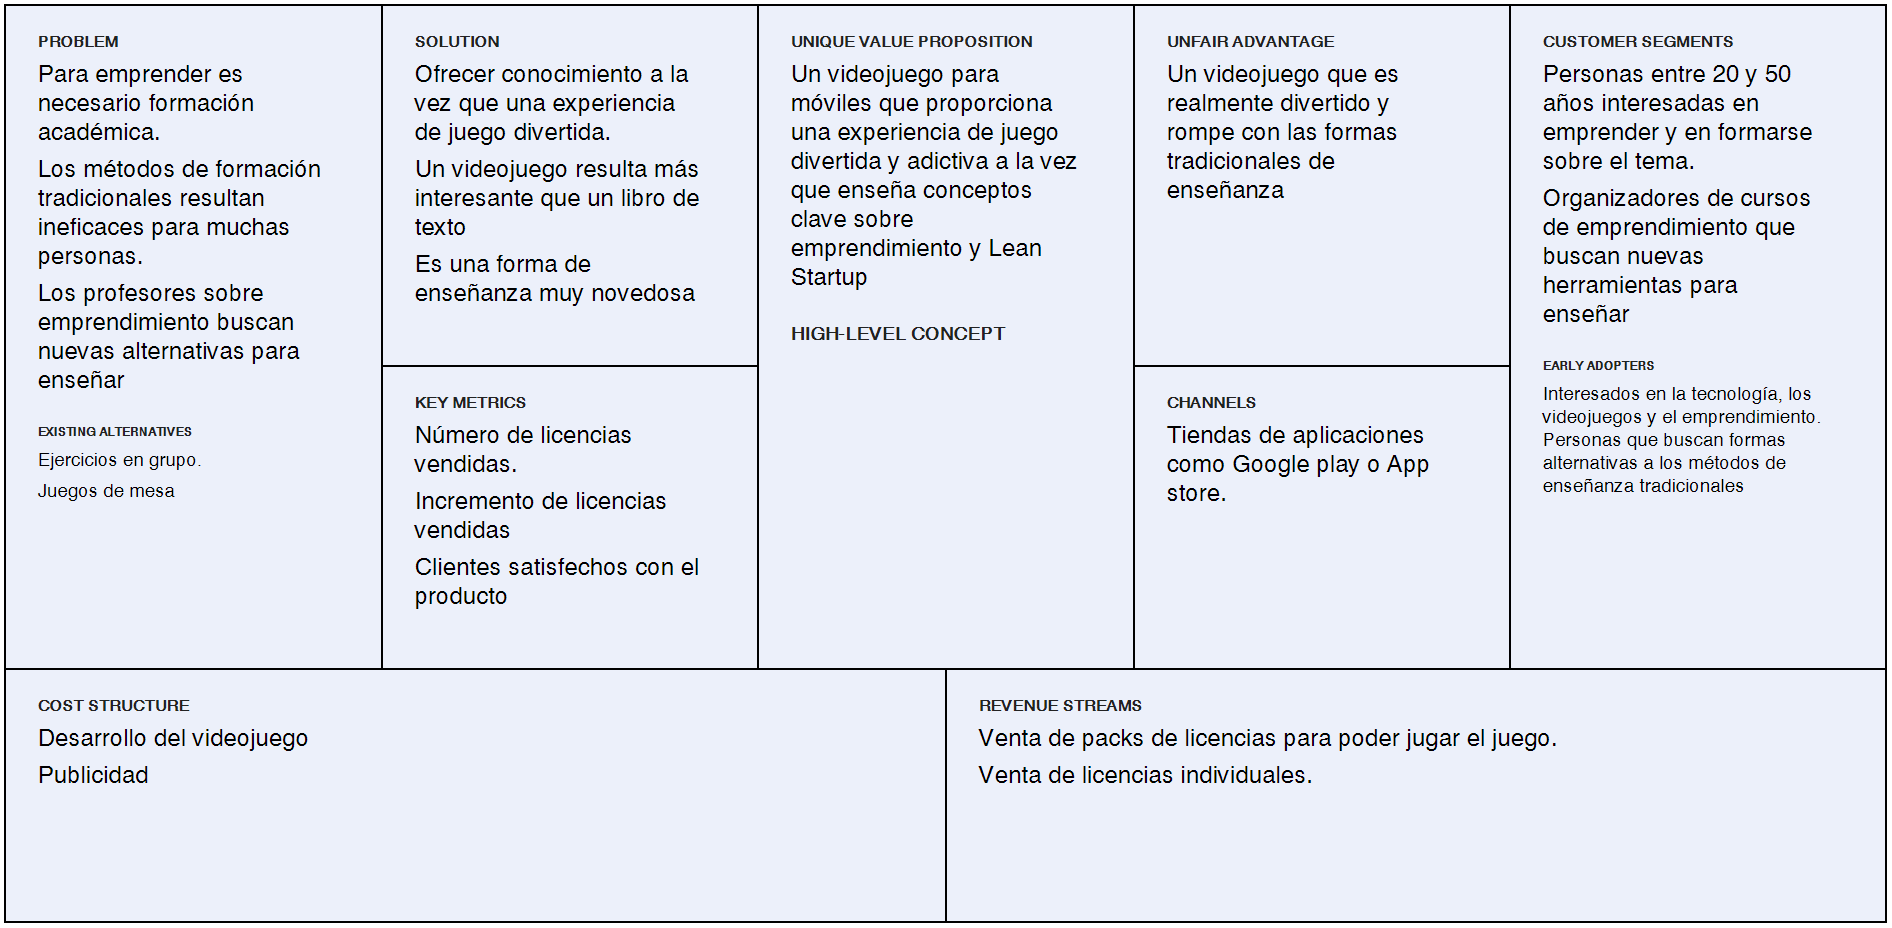
\includegraphics[scale=0.33]{imagenes/leanCanvasDaVinciStartup.png}
\caption{Lean canvas propuesto para este proyecto}
\label{leanCanvasDaVinci}
\end{center}
\end{figure}



